%% CAPITULO 2
\hypertarget{estilo:capitulo}{}
\chapter{REVISÃO BIBLIOGRÁFICA}

\section{A América do Sul}
\label{ss:americadosul}

Situada entre os oceanos Pacífico e Atlântico e meridionalmente entre a faixa tropical de latitudes de 10ºN e 60ºS e entre as longitudes de 70ºW e 30ºW, a AS é uma região de tempo e clima variados, com características tropicais, extratropicais e subtropicais \cite{satyamurtyetal98}. A AS é também uma região sobre a qual atuam diversos tipos de sistemas atmosféricos reguladores do tempo e do clima. Dentre eles, pode-se citar: 

\begin{itemize}
\item \textbf{Zona de Convergência do Atlântico Sul (ZCAS)}: banda de nebulosidade com orientação noroeste-sudeste e dominante nos meses de verão. Importante pelo regime de precipitação no continente com acumulados que podem chegar a $\sim$400 mm/mês \cite{kodama92};
\item \textbf{Zona de Convergência Intertropical (ZCIT)}: banda de nebulosidade com orientação equatorial, cuja posição varial sazonalmente entre as latitudes de 14ºN e 5ºS. É o mais importante sistema meteorológico a\-tu\-an\-te na região equatorial e que contribui para a precipitação na região norte do Nordeste do Brasil \cite{hastenrathheller77}, \cite{uvonobre89a}, \cite{uvonobre89b};
\item \textbf{Jatos de Baixos Níveis (JBN)}: um dos componentes do sistema de monção do continente. Importante pelo transporte de umidade proveniente da bacia Amazônia para a bacia do Paraná-Prata, ao sul e sudeste do continente alimentando os sistemas convectivos a leste dos Andes \cite{bonner68};
\item \textbf{Jato Polar (JP) e o Jato Subtropical (JST)}: jatos em altos níveis que são importantes devido à influência que exercem na propagação de frentes atmosféricas e na formação de alguns sistemas convectivos. São sistemas característicos onde a componente zonal do vento atinge valores máximos e geralmente estão associados à célula de circulação de Hadley (JST, mais regular) e ao gradiente horizontal de temperatura (JP, menos regular). São dominantes ao sul do continente, entre as latitudes de 35ºS a 70ºS (JP) e  20ºS a 35ºS (JST) \cite{reiter69}, \cite{riehl69};
\item \textbf{Alta da Bolívia (AB)}: outro componente do sistema de monção da AS. É um anticiclone da alta troposfera dominante no verão cuja manutenção é dada, basicamente, pela liberação e distribuição de calor pelo continente e ao longo do cinturão tropical. Este sistema é importante pela sua interação com outros sistemas meteorológicos como frentes atmosféricas e o Cavado do Nordeste (CN) \cite{carvalho89}, \cite{oliveira86};
\item \textbf{Baixa do Chaco (BC)}: é também um componente do sistema de monção do continente. Caracteriza-se por um sistema de baixa pressão, constante durante todo o ano sobre o norte da Argentina e o oeste do Paraguai. Atua com maior intensidade durante o verão \cite{grimmetal04}.;
\item \textbf{Cavado do Nordeste (CN)}: é também um vórtice ciclônico da alta troposfera. Sua formação está associada com a interação que tem com à incursão de baixas frontais ao sul-sudeste do continente.
\end{itemize}

Além disso, massas de ar e frentes atmosféricas entram e saem com frequência do continente devido à sua proximidade com o continente Antártico. O deserto do Atacama, a cordilheira dos Andes, a floresta Amazônica e o Nordeste brasileiro, também são exemplos da diversidade de cenários que compõem a AS - \autoref{fig02}.

\begin{figure}[!hbp]
\centering
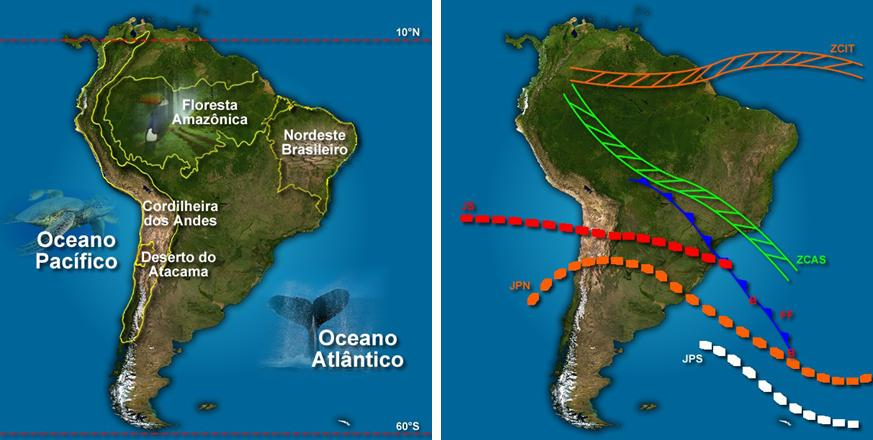
\includegraphics[height=7.5cm]{./figs/fig02.png}
\caption{Os principais cenários e sistemas atmosféricos da América do Sul.}
\label{fig02}
\end{figure}

Em termos de temperatura e precipitação, AS apresenta características bem distintas em regiões diferentes. Na região Amazônica, observa-se um clima chuvoso e de característica equatorial sem estação seca e com pequena flutuação térmica ao longo do ano. No extremo sul do continente, o clima é de latitudes médias com grande flutuação térmica. Além disso há a estação chuvosa durante o inverno (\-de\-vi\-do à incursão de frentes frias) e a estação seca durante o verão. A região Nordeste da AS possui clima com características de regiões semi-áridas, com estação chuvosa distribuída entre poucos meses ao longo do ano e com baixos níveis pluviométricos. Ao sul o clima possui características de subtrópicos, com estação seca bem definida no inverno e chuvosa no verão, com precipitação do tipo convectiva. Também, o clima da região sul é influenciado pelos climas das regiões de latitudes médias e trópicos.

Toda essa variedade de sistemas ambientais e meteorológicos em um continente situado numa zona tropical do globo é, basicamente, consequência direta dos diferentes regimes de precipitação presentes na região. 

A circulação atmosférica de grande escala possui um papel importante na circulação dos ventos e na distribuição de energia sobre a região dos trópicos. Nesta região há excesso de energia, diferentemente das regiões polares onde há déficit. O próprio fluído atmosférico, através de movimentos horizontais e verticais, redistribui este energia favorecendo o balanço térmico entre as diferentes regiões. Estes movimentos, que são contínuos, são mecanismos importantes da circulação de grande escala. É através deles que o ar sobe e desce, formando nuvens profundas e ocasionando a precipitação. Próximo à região equatorial, o ar sobe e desce nos subtrópicos por meio da célula de Hadley. As nuvens que se formam a partir desse processo, trazem precipitação convectiva para o norte do continente. Ao sul do continente, e diferentemente do que ocorre ao norte, os sistemas de baixa pressão favorecem o deslocamento das massas de ar e a formação das frentes frias. O choque térmico entre as massas de ar frias provenientes do continente antártico e de ar quente do continente sul-americano, causa chuvas e temporais. A umidade trazida da região amazônica pelos JBNs, também contribuem para a formação de sistemas convectivos que, em diferentes escalas, contribuem para os acumulados de precipitação do continente.

Na próxima seção, como continuação da apresentação dos aspectos que envolvem a área de estudo deste trabalho, é apresentada uma revisão sobre os Complexos Convectivos de Mesoescala.

\section{Comlpexos Convectivos de Mesoescala}
\label{ss:ccm}

Grande parte dos regimes de chuva observados sobre os trópicos e em especial, sobre a AS, é proveniente de um conjunto de sistemas meteorológicos precipitantes denominados Sistemas Convectivos de Mesoescala (SCMs). Os SCMs são importantes fenômenos meteorológicos cuja principal característica é a sua organização convectiva em diversas formas, mas com escala espacial da ordem de milhares a centenas de milhares de quilômetros de extensão.

Os Complexos Convectivos de Mesoescala (CCMs) são uma categoria de SCM e assim como as Linhas de Instabilidades, são conhecidos por serem um tipo extremo de SCM. Os CCMs são importantes fenômenos atmosféricos causadores de tempo severo e que contribuem significativamente para a variação dos níveis pluviométricos, principalmente sobre as regiões tropicais e de latitudes médias. Em meteorologia o termo ``tempo severo'' é habitualmente empregado para caracterizar situações de tempo sob as quais podem ocorrer uma série de eventos extremos, tanto em escala local quanto em escalas maiores. Estes eventos podem estar associados a chuvas muito fortes, intensas rajadas de ventos, descargas elétricas atmosféricas, granizo e até tornados \cite{maddox80}, \cite{menezessilvadias04}.

Os CCMs são sistemas convectivos que produzem alterações significativas na dinâmica de mesoescala, sendo na geração e redistribuição de calor latente, nas alterações de estabilidade vertical, remoção e redistribuição de umidade e, principalmente, na quantidade de radiação que entra e sai da atmosfera, devido à cobertura de nuvens associadas a esses sistemas.

Historicamente, a primeira definição formal de CCM foi introduzida por \citeonline{maddox80} para o Hemisfério Norte (HN). Mais tarde outros autores utilizaram esta definição para estudar outros casos de CCMs em partes diferentes do globo, como \citeonline{velascofritsch87}, na América do Sul. Segundo os critérios de \citeauthoronline{maddox80}, os CCMs podem ser classificados de acordo com suas características físicas: forma, tamanho e ciclo de vida. Quanto à forma, o CCM deve ser de formato circular, com excentricidade maior do que 0,7 (considerando-se a razão entre o eixo menor e o eixo maior - \autoref{fig08}). Quanto ao tamanho, o CCM deve apresentar uma cobertura de nuvens com temperaturas no infravermelho menores do que -32ºC e com área de 100.000 km². Na região mais interna da nuvem, as temperaturas devem ser mais frias (menores do que -52ºC) e com área em torno de 50.000 km². Quanto ao ciclo de vida, o CCM deve apresentar as características de tamanho persistentes a um período superior a 6 horas.

Todas estas características são semelhantes em escalas espaciais meso-a (ou meso-$\alpha$, de 250 a 2500 km de extensão e escala de tempo de 6 horas) e meso-b (ou meso-$\beta$, de 25 a 250 km de extensão e escala de tempo inferior a 6 horas).

Tipicamente, os CCMs são caracterizados por um conjunto de nuvens do gênero \textit{Cumulonimbus} cobertas por uma camada densa de nuvens do gênero \textit{Cirrus} e são facilmente identificados em imagens de satélites \cite{silvadias87}. O ciclo de vida dos CCMs é habitualmente noturno, ou seja, sua máxima extensão ocorre durante a madrugada \cite{velascofritsch87}, sendo o fim desse ciclo na metade do dia subsequente. Estas características dos CCMs tropicais e subtropicais são semelhantes em ambos os hemisférios (HN e HS).

\begin{table}[!hbp]
\caption{Resumo das características dos CCMs.}
\label{tab03}
\centering
\begin{tabular}{c|p{12cm}l}
\hline
\multicolumn{2}{c}{Caractarísticas}                                                 \\
\hline
Forma                                       & Circular: excentricidade maior do que 0,7.\\
\hline
\multirow{4}{2cm}{Tamanho}                  & Nuvens: topo com temperaturas \\
                                            & inferiores a -32ºC e cobertura \\
                                            & com área de $\sim$ 100.000 km²; \\
                                            & Parte interna: temperaturas inferiores a -52ºC e área de 50.000 km².         \\
\hline
\multirow{3}{2cm}{Ciclo de Vida}            & As características do tamanho devem persistir por mais do que 6 horas;   \\
                                            & Habitualmente noturno, com máxima extensão na madrugada.                \\
\hline
\multirow{3}{2cm}{Escala}                   & Meso-$\alpha$: 250 a 2500 km de extensão e escala de tempo de 6 horas;      \\
                                            & Meso-$\beta$: 25 a 250 km de extensão e escala de tempo inferior a 6 horas. \\
\hline
\multirow{4}{2cm}{Locais de Ocorrência} & Estados Unidos (HN);                  \\
                                            & Pacífico Oeste (HN);              \\
                                            & África (HS);                      \\
                                            & América do Sul (HS);              \\
\hline
\end{tabular}
\end{table}

\begin{figure}[!hbp]
\centering
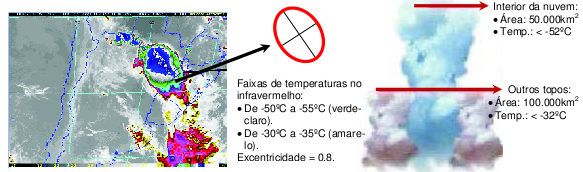
\includegraphics[height=4.5cm]{./figs/fig08.png}
\caption{À esquerda: imagem no infravermelho do satélite GOES (20030123, às 02:09 UTC). Ao centro: característica da excentricidade do CCM ocorrido nesta data. À direita: corte esquemático da nebulosidade durante um CCM.}
\FONTE{\citeonline{rozante08}}
\label{fig08}
\end{figure}

No Brasil, os CCMs ocorrem mais frequentemente na região Sul, havendo também referências de se deslocarem para as regiões Sudeste e Centro-Oeste, podendo ocorrer em todas as estações do ano \cite{silvadias96}. Na \autoref{fig09}, estão assinaladas as regiões Centro-Oeste (CO), Sudeste (SE) e Sul (SU) sob o domínio da AS. Estas são as regiões onde são observados com maior frequência a ocorrência de CCMs sobre a AS.

\begin{figure}[!hbp]
\centering
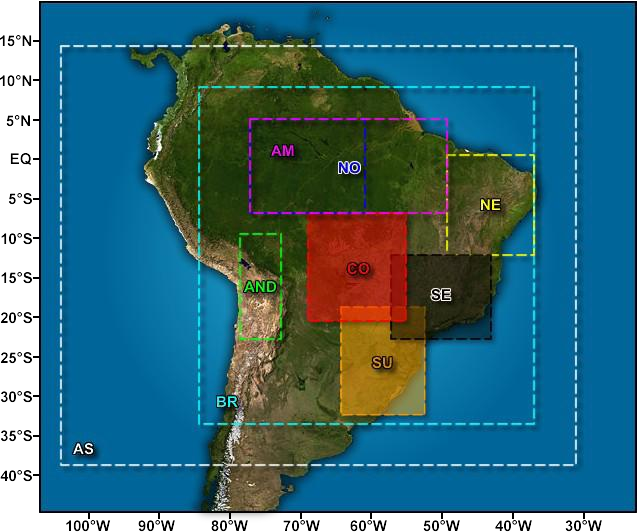
\includegraphics[height=10cm]{./figs/fig09.png}
\caption{Áreas de ocorrência de CCMs na AS.}
\label{fig09}
\end{figure}

Na AS, os principais mecanismos de transporte de umidade da região amazônica para a região sul da AS, são a ZCAS e o JBN. O JBN é o principal mecanismo associado à formação e alimentação da convecção de grande parte dos SCMs \cite{ferreiraetal03}, \cite{herdiesetal02}. O transporte de umidade da região amazônica em direção à região sul da AS, geralmente condensa e precipita na região de saída do JBN, produzindo fortes correntes descendentes sob o núcleo dos CCMs, com o máximo de precipitação durante a noite \cite{noguespaegleberbery00}. Esta característica é predominante em meses de verão, sendo que em meses de inverno, boa parte da umidade que condensa e precipita sobre o sul do continente é transportada pelos ventos alísios no norte do nordeste do continente. Na \autoref{fig10} é mostrado um modelo conceitual dos JBN e sua associação com a formação dos CCMs \cite{marengoetal04}.

\begin{figure}[!hbp]
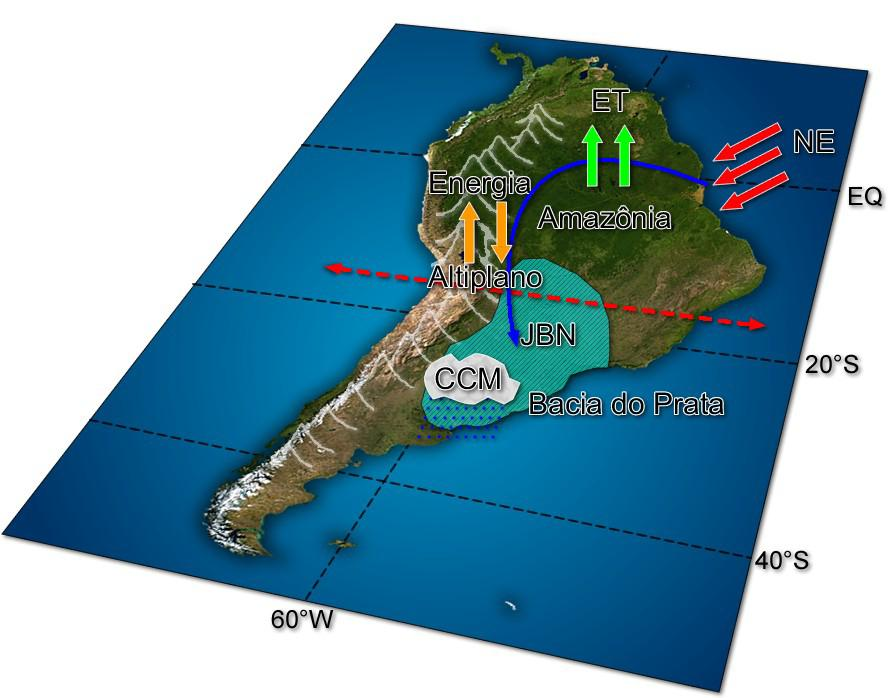
\includegraphics[height=10cm]{./figs/fig10.png}
\caption{Modelo Conceitual dos JBN. Na figura: ET - evapotranspiração do vapor d'água da floresta mazônica; JBN - Jato de Baixos Níveis que transportam a umidade e CCM - Complexo Convectivo de Mesoescala; NE - Ventos Alísios no norte do nordeste do continente.}
\FONTE{adaptado de \citeonline{marengoetal04}}
\label{fig10}
\end{figure}

No tópico a seguir, é feita uma introdução ao assunto de Assimilação de Dados e uma breve revisão histórica sobre o seu desenvolvimento.

\section{Assimilação de Dados}
\label{ss:assimdados}

Na modelagem atmosférica, o aprimoramento da Previsão Numérica de Tempo (PNT) de curto e médio prazo depende não somente do poder computacional envolvido - supercomputadores cada vez mais rápidos e eficientes (que permitem calcular as previsões de tempo mais rapidamente ou mesmo aumentar a resolução dos modelos), mas principalmente de fatores como o conhecimento exato das leis que governam o fluxo da atmosfera, da quantidade de dados observacionais e da determinação do estado inicial da atmosfera.  Embora não se tenha um conhecimento total sobre estas leis e condições - pois a atmosfera possui uma previsibilidade limitada devido ao seu comportamento caótico, os modelos de PNT são fundamentados na estrutura básica da atmosfera (leis de conservação de movimento, termodinâmica e continuidade - \autoref{form01}, \autoref{form02} e \autoref{form03}, respectivamente). Desta forma, tais modelos mantêm forte dependência em relação às condições do estado inicial da atmosfera - um importante fator que torna possível a previsão numérica de tempo mais acurada. Este fator, a condição inicial, também chamada de análise na assimilação de dados, é determinante para a PNT: quanto mais completo for - quanto mais informações possuir sobre o fluxo da atmosfera em seu instante de análise, mais preciso (acurado) será o resultado da previsão. (Convenciona-se, a partir daqui, que os vetores são denotados em negrito e as matrizes em letras maiúsculas).

\begin{equation}
\frac{d\textbf{\textit{v}}}{dt}+\textbf{\textit{v}}\cdot\nabla\textbf{\textit{v}}+2\mathbf{\Omega}\times\textbf{\textit{v}}=-\frac{1}{\rho}\nabla{p}+\textbf{\textit{g}}+\textbf{\textit{f}}
\label{form01}
\end{equation}

\begin{equation}
\frac{d\rho}{dt}+\nabla\cdot(\rho\textbf{\textit{v}})=0\rightarrow\frac{d\rho}{dt}=-\nabla\cdot(\rho\textbf{\textit{v}})
\label{form02}
\end{equation}

\begin{equation}
\frac{D\textit{e}}{D\textit{t}}=-\rho\frac{D\alpha}{D\textit{t}}+\textit{Q}
\label{form03}
\end{equation}

Onde:

\begin{itemize}
\item \textbf{\textit{v}}: é o vetor velocidade do fluido atmosférico em três dimensões, num referencial rotacional;
\item $\mathbf{\Omega}$: é o vetor tridimensional velocidade angular (velocidade com a qual o referencial rotacional se move);
\item $\rho$: é a densidade do fluido atmosférico;
\item \textit{p}: é a pressão do fluido atmosférico;
\item \textbf{\textit{g}}: é o vetor aceleração gravitacional em três dimensões;
\item \textbf{\textit{f}}: representa o vetor tridimensional da força de atrito (entre a atmosfera e a superfície terrestre);
\item \textit{e}: é a energia interna específica, que é uma função da temperatura do sistema;
\item \textit{Q}: é calor por unidade de massa;
\item $\alpha$: volume específico do fluido atmosférico. 
\end{itemize}

O processo de previsão numérica do tempo pode ser entendido como um problema de valor inicial e de contorno, no qual as equações governantes são integradas no tempo. As condições iniciais determinam como o modelo de previsão iniciará o ciclo de análise (\autoref{form01}). As condições de contorno determinam como serão os ciclos de previsão (\autoref{form02}), sendo portanto, muito importantes durante todo o tempo de integração do modelo \cite{nowosad01}. Para tanto, utilizam-se como condição inicial valores bem determinados dos campos meteorológicos em um dado instante de tempo e como condição de contorno, valores compatíveis em física e dinâmica com o modelo de previsão. Segundo \citeonline{talagrand97}, a AD pode ser definida como a forma mais acurada possível de se reconstruir o fluxo atmosférico utilizando todas as informações disponíveis no momento de sua geração. 

\begin{equation}
\textit{\textbf{w}}^{f}_{n}=\textit{\textbf{F}}[\textit{\textbf{w}}^{a}_{n-1}]
\label{form04}
\end{equation}

\begin{equation}
\textit{\textbf{w}}^{f}_{a}=\textit{\textbf{w}}^{f}_{n}+\textit{\textbf{d}}_{n}
\label{form05}
\end{equation}

Onde:

\begin{itemize}
\item $\textit{\textbf{w}}_{n}$: representa o vetor de variáveis de estado no passo temporal \textit{n};
\item $\textit{\textbf{F}}[.]$: representa o modelo de PNT;
\item $\textit{\textbf{d}}_{n}$: é o vetor de inovação da análise, o qual contém informações derivadas das observações.
\end{itemize}

Os índices $\textit{f}$ e $\textit{a}$ denotam os valores previstos e analisados, respectivamente.

A condição inicial utilizada nos modelos de PNT é constituída por um conjunto de observações, convencionais (de superfície e ar superior) e não convencionais (de satélites), as quais são providas nos quatro horários sinóticos padrões (00Z, 06Z, 12Z e 18Z) e por um campo de \textit{first guess} - uma previsão de curto prazo de tipicamente 6 horas. Todas estas informações são combinadas de forma ótima e constituem a análise que é a condição inicial dos modelos de PNT. Operacionalmente no CPTEC, essas observações são utilizadas nos horários das 00Z e 12Z (\autoref{fig03}). Estes são os horários em que as observações são mais abundantes sobre a AS e em que são feitas as previsões operacionais do centro. 

Mesmo havendo um grande número de observações sinóticas sobre a AS, há o problema da limitação de dados observados e disponíveis para a inicialização dos modelos de PNT. Sobre a AS, que está situada no Hemisfério Sul (HS), as porções de mares e oceanos são maiores do que as porções de terras e continentes. Esta situação é contrária ao que ocorre no Hemisfério Norte (HN). Nesta parte, a cobertura de radiossondagens e de equipamentos de monitoramento atmosférico sobre os continentes compõem uma estrutura densa muito mais eficiente de observações. Segundo \citeonline{morel80} e \citeonline{kalnay03}, em um período de aproximadamente 3 horas, a quantidade de informações coletadas (sobre a superfície, atmosfera, mares e oceanos) é insuficiente para iniciar um modelo de Equações Primitivas. Esta diferença, em relação ao número de graus de liberdade (considerando-se as variáveis e seus parâmetros) desse tipo de modelo, pode chegar a ser de uma ou até duas ordens de magnitude. Este fato indica que atualmente, com modelos mais sofisticados e a altas resoluções, existe uma necessidade muito maior de mais observações. Na prática, este tem sido um dos grandes desafios para a PNT. 

Sobre a AS, em uma janela de 6 horas (para os horários das 00Z e 12Z), há \-a\-pro\-xi\-ma\-da\-men\-te 10³ observações convencionais (\autoref{fig03}), das quais 45\% são observações de radiossondas (pontos em azul claro), 1,5\% são informações de navios (altura geopotencial - pontos vermelhos), 48\% são observações SYNOP (altura geopotencial - pontos azuis), 4\% são observações de boias (altura geopotencial - pontos amarelos) e 1,4\% são observações de aviões (vento - pontos verdes). Para os horários das 06Z e 18Z, a quantidade de observações é sensivelmente menor: há aproximadamente 10² observações (uma ordem de magnitude menor do que nos horários das 00Z e 12Z), sendo 0\% de radiossondas, 5\% de navios (altura geopotencial), 69\% SYNOP, 18\% bóias e 7,5\% de informações de vento advindas de aeronaves.

\begin{figure}[!hbp]
\centering
\includegraphics[height=20cm]{./figs/fig03.png}
\caption{Observações convencionais sobre a AS para o dia 28 de setembro de 2009, assimiladas pelo sistema RPSAS. Observações válidas para os horários das 00Z e 12Z (primeira linha) e para o horário das 06Z e 18Z (segunda linha).}
\FONTE{<\url{http://assimila.cptec.inpe.br}>}
\label{fig03}
\end{figure}

Na AD, apesar de as observações sinóticas serem a principal fonte de informações sobre o fluxo da atmosfera, estas podem apresentar algumas deficiências. Segundo \citeonline{morel80}, em uma situação física ideal, pode-se esperar que as observações (que são informações sinóticas) determinem um valor para cada parâmetro meteorológico (e.g. temperatura, pressão à superfície e ventos, que são quantidades físicas). No entanto, observa-se que isto não acontece devido a vários fatores:

\begin{itemize}
\item As observações de temperatura, pressão à superfície e ventos são distribuídas de forma muito irregular e há muitas dúvidas sobre as regiões onde não há observações;
\item As observações convencionais são medidas pontuais que podem não ser representativas dos campos meteorológicos de volumes médios, tal como os modelos de PNT requerem.
\end{itemize}

Além disso, observações convencionais estão sujeitas a erros grosseiros dos instrumentos de medição. Por outro lado, temos as observações não convencionais (que são informações assinóticas ou remotas), as quais podem fornecer mais detalhes sobre o fluxo atmosférico e que complementam as informações providas pelas observações sinóticas. 

No entanto, estes tipos de observações também possuem as suas limitações:

\begin{itemize}
\item As observações não convencionais podem, por exemplo, fornecer informações sobre perfis verticais de temperatura. Estes perfis são determinados a partir do espaço e de forma remota, provendo uma cobertura contínua e homogênea em um período de tempo de 6 a 12 horas. Emmbora estas observações sejam assinóticas, elas têm a vantagem de ser distribuídas (de forma contínua) no tempo e no espaço. No entanto, os satélites que fornecem essas observações, são síncronos com o Sol tornando o seu aproveitamento pelos modelos de PNT, incompleto;
\item Os satélites geoestacionários são capazes de disponibilizar observações remotas do movimento das nuvens e prover uma amostragem horizontal dos campos de vento nos quatro horários sinóticos padrões. No entanto, a resolução vertical dessas observações pode ser limitada a poucos níveis verticais, o que também pode fazer com que o seu aproveitamento pelos modelos de PNT seja incompleto.
\end{itemize}

Estes tipos de observações, sempre incluem considerações físicas e algoritmos sofisticados para reconstruir os parâmetros meteorológicos, a partir de quantidades medidas remotamente. Estes procedimentos também têm a sua própria deficiência e podem causar erros aleatórios e/ou sistemáticos.

Desta forma, pode-se concluir que o conjunto de dados que se tem disponível para uso com os modelos de PNT, pode ser incompleto e insuficiente para uma descrição detalhada e adequada do fluxo atmosférico global. Por outro lado, o uso combinado de observações convencionais e não convencionais, mostra-se muito interessante por formar um conjunto de dados mais consistente para uso como validação dos modelos e como condição inicial nos modelos de PNT. 

No CPTEC, operacionalmente utilizam-se observações sinóticas e assinóticas para a assimilação, as quais são interpoladas na grade dos modelos utilizando-se um sistema de análise estatística em espaço físico (espaço das observações). No caso regional, atualmente são assimiladas observações convencionais provenientes do \textit{Global Telecommunication System} (GTS) e observações não convencionais como, por exemplo, dados de altura geopotencial e água precipitável provenientes do sistema de sondagens remota \textit{Atmospheric Infrared Sounder/Advanced Microwave Sounding Unit} (AIRS/AMSU); dados de vento sobre o oceano \textit{Quick Scaterometer} (\textit{QuikScat}); dados de vento de satélite, a partir do deslocamento de nuvens \textit{Clod Track Wind} (\textit{CTW}) entre outros. Como exemplo, \citeonline{andreolietal07} mostram que, apesar da baixa quantidade de informações sobre o HS, as sondagens AIRS/AMSU são de fundamental importância para uma boa previsão de tempo sobre a AS. Neste contexto, o uso de observações não convencionais providas por satélites em uma região do globo onde sabe-se que há uma grande carência de observações, contribui em grau elevado para o aprimoramento do desempenho da PNT. Nesta dissertação de mestrado, propõe-se o uso das informações das taxas de precipitação providas pelo satélite \textit{Tropical Rainfall Measuring Mission} (TRMM) como forma de contribuir para que esse grau de aproveitamento do uso de observações de satélites sobre a região seja elevado.

Qualquer modelo de PNT precisa ser inicializado (ou iniciado) mesclando-se as observações com campos estimados atuais, calculados com base em observações de um instante de tempo passado. Formalmente, este problema consiste em otimizar a integração do modelo (considerando-o como um sistema com $n-1$ graus de liberdade e $n$ variáveis, ou seja, considerando-se as variáveis em questão e os parâmetros associados a elas), enquanto adicionam-se todas as informações atuais disponíveis. Esse processo de mesclar-se as novas observações com o resultado da integração do modelo de PNT é conhecido como Assimilação de Dados Quadrimensional ou \textit{Four Dimensional Dada Assimilation} (4DDA), em consideração à base espaço-temporal dos dados (latitude, longitude, níveis verticais de pressão e o tempo).

Historicamente, o desenvolvimento das metodologias de AD e 4DDA passou por três estágios principais \cite{wangetal00}, e \cite{kalnay03}:

\begin{itemize}
\item \textbf{Análise Simples:} um estágio muito inicial durante década de 1950, enquanto não havia computadores suficientemente rápidos. Os métodos de Análise Simples foram as bases da AD moderna. Nesta década a Análise Simples envolvia técnicas simples de interpolação de dados como Correções Sucessivas, Relaxação Newtoniana e \textit{Nudging}. Nestas abordagens, utilizam-se os dados observados para forçar (\textit{nudge}) o modelo a produzir um estado próximo ao do que a observação representa;
\item \textbf{Interpolação Ótima (IO):} considerações estatísticas (baseadas na Teoria da Estimação) foram introduzidas na análise atmosférica e na AD, durante as décadas de 1960 e 1970. Baseadas nestas considerações, métodos baseados em IO foram utilizados para assimilar dados observados em modelos de PNT. Tais métodos de IO foram muito utilizados em vários centros operacionais ao redor do mundo;
\item \textbf{Análise Variacional:} nas décadas de 1980 e 1990 os métodos de assimilação foram substituídos por métodos variacionais como os sistemas de análise multivariacionais (3DVAR, em três dimensões e o 4DVAR em quatro dimensões) utilizando modelos adjuntos. Estas técnicas foram uma evolução das técnicas utilizadas nas décadas passadas e, mais modernas, ainda são largamente utilizadas nos centros operacionais de PNT; 
\item \textbf{Teoria da Estimação:} no início da década de 1960 o Filtro de Kalman (FK) foi amplamente utilizado para se estimar o estado de um modelo a partir de medidas que continham imperfeições (ruído). Este método tem aplicação desde a economia, passando pela robótica até a geofísica de fluídos dinâmicos. Décadas mais tarde, modelos baseados no FK foram aplicados em modelos geofísicos com diversos membros (previsão por conjunto - \textit{ensemble}). Esta nova abordagem foi introduzida por \citeonline{evensen94}, \citeonline{evensen03} e considera que os membros do modelo possuem uma distribuição de probabilidades Gaussiana. Outros \textit{approachs} do FK incluem: EnSRF \cite{andres68}, \cite{withakerhamill02}; EAKF \cite{anderson01}; ETKF \cite{bishopetal01}; EnKF \cite{kalnay04}; ETKF \cite{kalnay03} e o LETKF \cite{hunt05}.
\item \textbf{Inteligência Artificial:} recentemente, o uso da Inteligência Artificial tem sido aplicado à AD por meio de Redes Neurais \cite{nowosad01}. Este novo tipo de abordagem tem sido estudado e aplicado em alguns modelos, mas não se tem notícias de seu uso operacional.
\end{itemize}

Em geral, o \textit{approach} destas técnicas é combinar, de forma ótima, as informações de observações e \textit{first guess}, calculando os peses necessários dos erros das observações para produzir a melhor estimativa possível da condição inicial do modelo.

Todos esses esquemas de assimilação evoluíram de acordo com o poderio computacional desenvolvido e adquirido ao longo do tempo. Embora a teoria estatística, que serve de base para praticamente todos os esquemas de AD, já existisse, foi o desenvolvimento de computadores e arquiteturas mais velozes que permitiram a paralelização e otimização dos esquemas. Este desenvolvimento também possibilitou que a AD fosse desenvolvida no ramo da previsão por \textit{ensemble} (por conjunto) e também na geração dos algoritmos utilizados por este tipo de esquema.

\section{Ciclo de Assimilação de Dados}
\label{ss:cicloassimdados}

O Ciclo de Assimilação de Dados (CAD) pode ser definido como um sistema \-re\-tro\-a\-li\-men\-ta\-dor (ou de \textit{feedback}) que obtém uma nova análise a partir de informações previamente inseridas no modelo. Como visto anteriormente, há vários métodos de AD e, portanto, diferentes esquemas utilizados em diversos centros operacionais de PNT.

De forma geral, o CAD, pode ser dividido em 4 etapas comuns a todos os diferentes esquemas de assimilação \cite{nowosad01}:

\begin{itemize}
\item \textbf{Controle de Qualidade:} no início do CAD, são verificados os dados observados em termos de consistência da distribuição espaço-temporal. Os dados são comparados com os seus vizinhos e são verificados erros de codificação dos dados e de localização dos intrumentos de medição. Nesta etapa os dados podem ser rejeitados ou não;
\item \textbf{Análise Objetiva:} nesta etapa os dados observados são interpolados na grade do modelo e são feitas pequenas correções nos campos previstos do \textit{first guess}. Nesta etapa o \textit{first guess} é preparado para a geração da análise;
\item \textbf{Inicialização:} nesta etapa, a partir da análise, são calculadas as condições iniciais de integração as quais devem ser livres de oscilações ou ondas espúrias (e.g. ondas de gravidade inercial). Este processo consiste da utilização de um filtro, responsável pelo processo de inicialização  dos dados inseridos no modelo (mais adiante será feita uma introdução ao Filtro Digital (FD) do modelo EtaWS);
\item \textbf{Previsão de Curto Prazo:} nesta etapa é gerado o \textit{first guess} do próximo ciclo. Nesta etapa utiliza-se um sistema de assimilação para preparar o próximo estado do modelo. Este sistema inclui as parametrizações necessárias para assegurar que, se não for atualizado com novas observações, o estado por ele gerado será próximo do verdadeiro. Isto garante que na falta de dados, o \textit{first guess} produzido pelo sistema de AD permaneça plausível.
\end{itemize}

No processo de assimilação de dados, as informações são extraídas das observações - comumente esparsas, para reconstruir e/ou ajustar a estrutura das variáveis que representam os sistemas atmosféricos. A técnica combina um estado da atmosfera anteriormente predita por uma previsão de curto prazo, normalmente de 6 horas - (1A na \autoref{fig04} à esquerda), com dados observacionais recentes (1B na \autoref{fig04}), para produzir um estado atmosférico estimado e atualizado (análise - 4 na \autoref{fig04}) e que é usado como condição inicial a partir da qual se gera uma nova previsão.

A \autoref{fig04} representa o esquema de um CAD contínuo, onde mostradas as diferentes partes do esquema:

\begin{figure}[!hbp]
\centering
\includegraphics[height=7cm]{./figs/fig04.png}
\caption{CAD - Ciclo de Assimilação de Dados. Figura à esquerda: as etapas de um CAD. Figura à direita: exemplo do ciclo contínuo de assimilação de dados.}
\FONTE{Figura da esquerda, \citeonline{demattos06}.}
\label{fig04}
\end{figure}

\section{Sistema Regional de Análise Estatística em Espaço Físico (RPSAS)}
\label{ss:rpsas}

No CPTEC, o atual sistema operacional de AD é o \textit{Physical-space Statistical Analysis System} (PSAS) T213L42 - com 213 ondas no Equador ($\sim$ 60 km de resolução horizontal) e 42 níveis verticais, sendo sigma ($\sigma$) a coordenada vertical. No contexto regional, é utilizado o \textit{Regional Physical-space Statistical Analysis System} (RPSAS) que é derivado do sistema PSAS desenvolvido pela divisão de assimilação de dados da \textit{National Aeronautics and Space Administration} (NASA) \cite{dasilvaetal95}, \cite{courtier97}. Operacionalmente, o RPSAS é utilizado pelo CPTEC com 40 km de resolução espacial, para produzir a análise utilizada pelos modelos regionais do centro (Eta e \textit{Braziliam} RAMS (BRAMS)).

O sistema de assimilação de dados RPSAS é a versão regional desenvolvida e mantida pelo CPTEC em parceria com o \textit{Global Modeling and Assimilation Office} (GMAO) da NASA. O RPSAS utiliza o mesmo sistema de geração da análise do \textit{Global Physical-space Statistical Analysis System} (GPSAS) \cite{dasilvaetal95}, \cite{cohnetal98}. O RPSAS é considerado um esquema com características de 3DVAR e de IO, porém sem as limitações globais do algoritmo do 3DVAR. Estas características permitem que o sistema realize boa parte dos seus cálculos no local onde as observações se encontram e não globalmente, tornando o sistema computacionalmente mais econômico. 

O RPSAS é executado de forma experimental com 20 km de resolução espacial em conjunto com o modelo regional EtaWS principalmente para previsões de tempo de curto prazo. O sistema é capaz de utilizar dados convencionais provenientes do GTS, tais como SYNOP, TEMP, SATOB entre outros, além de dados de satélite (\textit{QuikSCAT}, TRMM, ATOVS e AIRS, como pode ser visto na seção anterior).

\section{Equação de Inovação e de Análise}
\label{ss:eqinovanl}

O RPSAS utiliza como núcleo de análise o próprio PSAS, sendo que as equações de análise e inovação são resolvidas para o caso regional. Para calcular as inovações trazidas pelas observações e como forma de calcular a análise, são utilizadas as seguintes equações (adaptado de \citeonline{larsonetal98}):

\begin{equation}
(HP^{f}H^{T}+R)X=\textit{\textbf{w}}^o-H\textit{\textbf{w}}^f
\label{form06}
\end{equation}

\begin{equation}
\textit{\textbf{w}}^a-\textit{\textbf{w}}^f=P^{f}H^{T}X
\label{form07}
\end{equation}

Em que:

\begin{equation}
X^{a}=X^{b}+W[y^{o}-H(X^{b})]
\label{form08}
\end{equation}

Onde:

\begin{itemize}
\item $P^{f}$: é a matriz (de ordem $n$) de covariância dos erros da previsão;
\item $R$: é a matriz (de ordem $p$) de covariância dos erros de observação;
\item $H$: é uma matriz de ordem $p$$\times$$n$ que interpola as observações na grade no vetor previsão (em ponto de grade);
\item $\textit{\textbf{w}}^o$: é o vetor das observações, de ordem $p$;
\item $\textit{\textbf{w}}^f$: é o vetor previsão (em ponto de grade), de ordem $n$;
\item $\textit{\textbf{w}}^a$: é o vetor análise, de ordem $n$;
\item $\textit{X}$: é a matriz de covariância dos erros de observação.
\end{itemize}

O lado direito da \autoref{form06} é chamado de Vetor Inovação ou Resíduo Observação Menos Previsão (\textit{Observation Minus Forecast} - OMF), e o lado esquerdo da \autoref{form07} é chamado de Incremento da Análise (AI - Analysis Increment). É importante observar que o PSAS ingere os dados observacionais através do vetor OMF na forma $\textit{\textbf{w}}^o-H\textit{\textbf{w}}^f$.

O PSAS resolve a \autoref{form06} e a \autoref{form07} sem formar explicitamente as matrizes $HP^{f}H^{T}$, $R$ e $P^{f}H^{T}$. A representação destas matrizes e a solução da \autoref{form06} e da \autoref{form07} podem ser encontradas em \citeonline{guoetal98}.

Em termos de custo computacional, como mencionado anteriormente, o PSAS é capaz de realizar os cálculos no ponto em que as observações de encontram. Considerando-se um sistema em que $n=10^{6}$ e $p=10^{5}$ (aproximadamente), arranjando-se e resolvendo-se a \autoref{form06}, o esforço computacional para o PSAS é reduzido pela metade (em relação ao 3DVAR). O resto do tempo de máquina é devido à transformação da matriz $X$ (da \autoref{form07}) das observações para o espaço das observações \cite{cohnetal98}.

De forma simplificada, o PSAS segue o seguinte algoritmo:

\begin{enumerate}
\item Construção da matriz $HP^{f}H^{T}+R$ e solução da \autoref{form06} para $X$;
\item Construção da matriz $P^{f}H^{T}$ da \autoref{form07} e cálculo do incremento da análise ($\textit{\textbf{w}}^a-\textit{\textbf{w}}^f$) a partir de $X$;
\item Cálculo da previsão e da matriz dos erros de covariância das observações (matriz $X$) para uso nos passos \textit{a} e \textit{b};
\item Particionamento (tipagem) e outros processamentos nos dados observacionais de entrada.
\end{enumerate}

Na seção a seguir, serão apresenados os componentes principais do sistema RPSAS.

\section{Componentes do Sistema de Assimilação de Dados RPSAS}
\label{ss:compsisassimdados}

\subsection{Modelo Regional EtaWS}

O modelo regional Eta Workstation (EtaWS) \cite{mesingeretal88}, \cite{black94} a ser utilizado nas \-si\-mu\-la\-ções é a versão pré-operacional utilizada no CPTEC para PNT com 20 km de resolução espacial e 38 níveis na vertical. Esta versão do modelo Eta foi escolhida para a realização dos experimentos por ser uma versão mais atual do modelo, que inclui um conjunto de física mais moderno e por ser utilizada com maior resolução. Além disso, esta versão do modelo EtaWS vem sendo utilizada em modo pesquisa acoplado com o sistema RPSAS há alguns anos pelo grupo de AD do CPTEC, sendo portanto, uma versão pré-operacional.

Basicamente, a diferença entre a versão operacional (Eta) e a versão pré-operacional (EtaWS) do modelo está na implementação física, que é mais completa no EtaWS (outras diferenças na \autoref{tab01} adiante). De forma geral, o modelo Eta se propõe a prever com detalhes sistemas organizados de mesoescala tais como SCMs, Sistemas Frontais, Brisas Marítimas, Tempestades e outros \cite{chou96}.

Como principais características, o modelo EtaWS pode ser utilizado nos modos hidrostático e não-hidrostático (quando considera os movimentos verticais) e com uma coordenada vertical eta ($\eta$) que, em comparação à coordenada sigma ($\sigma$), reduz os erros numéricos no cálculo da força do gradiente de pressão nas encostas de topografias íngremes. A \autoref{form09} define a coordenada vertical $\eta$:

\begin{equation}
\eta=\frac{(p-p_{top})}{(p_{s}-p_{top})}\bigg[\frac{p_{ref}(z_{0})-p_{top}}{p_{ref}(z_{s})-p_{top}}\bigg]
\label{form09}
\end{equation}

Onde:

\begin{itemize}
\item $p$: é a pressão;
\item $p_{top}$: é a pressão no topo do modelo;
\item $p_{s}$: é a pressão na superfície;
\item $p_{ref}$: é a pressão de referência sobre uma superfície $\eta$ no topo de uma montanha ($z_{s}$) e na base da mesma ($z_{0}$).
\item $\frac{(p-p_{top})}{p_{s}-p_{top}}=\sigma$ (coordenada sigma)
\end{itemize}

O modelo utiliza uma grade horizontal do tipo semi-alternada E de Arakawa \cite{arakawalamb77} e um esquema de integração temporal \textit{split-explicit} - no qual os modos associados à gravidade são tratados com um passo de tempo menor, 20 km de resolução espacial e 38 níveis verticais, com o topo do modelo a 25 hPa. Para uma melhor simulação dos processos próximos à superfície, o modelo possui 17 níveis verticais entre a superfície e o nível de 700 hPa. O domínio de integração do modelo regional cobre a maior parte da AS e parte dos oceanos Atlântico e Pacífico, aproximadamente entre as latitudes de 10ºN - 60ºS e entre as longitudes de 90ºW - 20ºW (\autoref{fig05}). 

\begin{figure}[!hbp]
\centering
\includegraphics[height=10cm]{./figs/fig05.png}
\caption{Topografia (sombreado colorido) e Domínio (sombreado cinza) de integração do modelo regional EtaWS com resolução horizontal de 20 km.}
\label{fig05}
\end{figure}

Em relação aos processos físicos, o modelo EtaWS possui um conjunto de física completa com parametrizações para precipitação convectiva rasa e profunda. O modelo utiliza o esquema de convecção \textit{Cumulus} Betts-Miller melhorado por Janjić (BMJ) \cite{betts86}, \cite{bettsmiller86}, \cite{janjic94}. 

O esquema BMJ considera apenas movimentos verticais ascendentes (convecção). O movimento convectivo transporta calor e umidade removendo ou reduzindo a condição de instabilidade da atmosfera (quando a atmosfera real é mais ou menos úmida do que a atmosfera de referência) alterando os perfis verticais de calor latente e umidade. A atmosfera de referência considera perfis de temperatura e umidade observados por \citeonline{betts86} e \citeonline{bettsmiller86}, que são relativamente secos e seguem adiabáticas úmidas. O esquema é acionado quando a atmosfera real é mais úmida do que a atmosfera de referência (ambiente condicionalmente instável).

Outro aspecto relevante do modelo EtaWS, é a parametrização de superfície. O esquema de superfície utilizado no EtaWS, inclui o modelo NOAH \textit{Land Surface Modelo} (NOAH LSM - \cite{mitchell01}). Esta versão do NOAH utilizada em conjundo com o modelo EtaWS inclui 16 classes diferentes de solo (entre 0 e 30 cm de profundidade) e 24 classes diferentes de vegetação (\autoref{fig06}). As tabelas com os nomes das classes de solo e vegetação do NOAH LSM podem ser encontrada no Anexo A deste trabalho).

\begin{figure}[!hbp]
\centering
\includegraphics[height=20cm]{./figs/fig06.png}
\caption{Classes de Solo e Vegetação do Modelo de Superfície NOAH.}
\label{fig06}
\end{figure}

Entre outros aspectos da física do modelo, pode-se citar:

\begin{itemize}
\item \textbf{Dinâmica:} Hidrostática ou Não-Hidrostática - o modelo pode ser executado com a coordenada vertical sendo a pressão ou a altura, respectivamente (nos experimentos, o modelo é ajustado para o modelo não-hidrostático);
\item \textbf{Turbulência:} Mellor-Yamada 2.5 para as trocas verticais na atmosfera livre (entre as camadas do modelo) e Mellor-Yamada 2.0 para as trocas entre a superfície e a camada mais baixa do modelo \cite{melloryamada74};
\item \textbf{Processos radiativos:} Lacis-Hansen para o cálculo da radiação de onda curta \cite{lacishansen74} e Fels-Schwarzkopf para o cálculo da radiação de onda longa \cite{felsschwarzkopf75};
\item \textbf{Nuvens:} esquema de microfísica de nuvens de Ferrier \cite{ferrieretal02}, onde podem ser estimadas nuvens altas, médias e baixas além de diversos tipos de hidrometeoros;
\item \textbf{Processos de Superfície:};
\item \textbf{Camada Limite:}.
\end{itemize}

A \autoref{tab01} resume as principais diferenças entre a versão operacional do modelo Eta e a versão pré-operacional EtaWS utilizada neste trabalho.

\begin{table}[!hbp]
\caption{Diferenças principais entre os modelos Eta e EtaWS.}
\label{tab01}
\centering
\begin{tabular}{c|c|c|c}
\hline
Característica                       &                         & Eta               & EtaWS              \\
\hline
\multirow{2}{2.8cm}{Dinâmica}        &                         & Hidrostática      & Hidrostática       \\
                                     &                         &                   & Não-Hidrostática   \\
\hline
                                     & Superfície              & OSU LSM           & NOAH LSM           \\ 
\multirow{2}{2.8cm}{Parametrizações} & Precipitação Convectiva & Betts-Miller      & Betts-Miller-Janjić\\
                                     &                         &                   & Kain-Fritsh        \\
                                     & Microfísica de Nuvens   & Zhao              & Ferrier            \\
\hline
\end{tabular}
\end{table}

O albedo e a fração de cobertura vegetal são obtidos a partir de climatologias globais sazonais e mensais, respectivamente. As condições iniciais ($u$, $v$, $t$, $q$, $p_{s}$ - ventos temperatura, umidade e pressão à superfície) no primeiro ciclo de assimilação de dados são as provenientes das análises do NCEP. Posteriormente, no processo cíclico de assimilação, as condições são fornecidas pelo próprio modelo EtaWS. As condições de contorno são provenientes do modelo global do CPTEC T126L28 e atualizadas a cada 6 horas. A temperatura do mar é obtida dos valores semanais e/ou mensais para o período de estudo com resolução 1ºx1º.

\subsection{Filtro Digital}

Nos primórdios da modelagem numérica do tempo e da PNT, modelos de equações simplificadas eram mais viáveis para a previsão numérica por serem mais simples e por ter um custo computacional menor. Modelos de equações primitivas envolviam um custo computacional muito maior, por serem mais complexos e por exigirem a utilização de um filtro para a inicialização dos dados inseridos no modelo. 

A análise e a inicialização são os componentes principais dos sistemas de AD. Segundo \citeonline{kasahara90}, os métodos de análise são desenhados para verificar os campos de massa e a componente rotacional do vento. Já os de inicialização são desenhados para obter a componente irrotacional do vento e o campo de velocidade vertical associado, os quais são balanceados com os campos de massa e são livres de oscilações de alta frequência. A teoria quase-geostrófica, métodos dos Modos Normais Não-Lineares (MNN) e outros produzem bons resultados em latitudes médias, mesmo sem considerar os efeitos diabáticos para movimentos de grande escala. Nos trópicos, entretanto, devido à pequena magnitude do parâmetro de \textit{Coriolis} e ao fraco gradiente horizontal de temperatura, a situação é diferente: os métodos de inicialização devem incluir os efeitos diabáticos, associados principalmente à precipitação. Uma forma de incluir esses efeitos é utilizar o método de \textit{nudging}. Nesse método os campos são gradualmente corrigidos sem que seja requerido nenhum outro processo de inicialização para se manter o balanço dinâmico - tal como ocorre com a Inicialização Física (IF) em que as ondas espúrias podem ser controladas por um FD (ajustado no próprio modelo de previsão). Isto é, onde as observações meteorológicas são inseridas, os termos artificiais das equações prognósticas são conduzidos em direção aos valores observados \cite{kalnay03}. 

O processo de inicialização consiste em acelerar o equilíbrio entre os campos de massa (componentes do vento) e velocidade (movimentos verticais) nos dados iniciais com o objetivo de se reduzir o ruído gerado que pode se propagar durante a integração do modeloe causar um desbalanço entre o modelo e os dados inseridos. 

\citeonline{harter99} enumera algumas causas desta desbalanço entre os campos de massa e velocidade nos dados iniciais:

\begin{enumerate}
\item Erros nos dados observados;
\item Imperfeições nos métodos numéricos que aproximam as equações diferenciais por equações em diferenças finitas;
\item Resolução horizontal do modelo;
\item Erros de representação dos termos não-lineares;
\item Erros de truncamento em modelos espectrais (modelos globais).
\end{enumerate}

Nos experimentos propostos nesta dissertação de mestrado, utiliza-se o FD original do modelo EtaWS, e que segue o esquema proposto por \citeonline{lynchhuang93}. A IFD no modelo EtaWS, consiste em integrar o modelo por 3 passos de tempo para trás e depois por 3 passos de tempo para frente (totalizando 6 passos de tempo). Em cada passo de tempo, e em cada ponto de grade, as variáveis prognósticas do modelo são filtradas, com a vantagem de ao final da integração, se obter uma Condição Inicial Filtrada (CIF). Esta CIF é a combinação das duas integrações feitas anteriormente (para frente e para trás). Em seguida, o modelo EtaWS utiliza esta CIF para fazer as previsões. Este procedimento é realizado no início da previsão e depois da geração da análise pelo RPSAS. O objetivo de se empregar a IFD é forçar o balanço dos campos de \textit{first guess} gerados pelo modelo EtaWS, quando houver a assimilação de precipitação.

A seguir é feita uma descrição dos ciclos de análise e previsão dos sistema EtaWS+RPSAS.

\subsection{Descrição do Ciclo EtaWS+RPSAS (Ciclos de Análise e Previsão)}

O ciclo de análise e previsõe do EtaWS+RPSAS está esquematizado na \autoref{fig07}. Neste esquema, a cada ciclo de 3 horas, é feita uma correção do \textit{first guess} assimilando-se a precipitação. Desta forma, a assimilação de precipitação é realizada durante a geração do \textit{first guess}, pelo modelo EtaWS. 

Na subseção a seguir, o esquema de assimilação de precipitação é explicado com mais detalhes.

\begin{figure}[!hbp]
\setlength{\unitlength}{1mm}
\begin{picture}(50,50)
\put(0,40){Ciclo de}
\put(0,35){Análise}
\put(0,12.5){Ciclo de}
\put(0,7.5){Previsão}
\put(0,25){\line(1,0){150}}
%\put(0,48){\line(1,0){150}}

\put(47.5,50){dia $n$}
\put(107,50){dia $n+1$}

\put(18,0){\line(0,1){50}}

\put(22.5,45){\oval(8,4)}
\put(19,43.5){00Z}
\put(22.5,43){\vector(0,-1){25}}

\put(31,45){\oval(8,4)}
\put(27.5,43.5){03Z}
\put(31,35){\vector(0,1){8}}

\put(39.5,45){\oval(8,4)}
\put(36,43.5){06Z}
\put(39.5,43){\vector(0,-1){25}}

\put(48,45){\oval(8,4)}
\put(44.5,43.5){09Z}
\put(48,35){\vector(0,1){8}}

\put(56.5,45){\oval(8,4)}
\put(53,43.5){12Z}
\put(56.5,43){\vector(0,-1){25}}

\put(65,45){\oval(8,4)}
\put(61.5,43.5){15Z}
\put(65,35){\vector(0,1){8}}

\put(73.5,45){\oval(8,4)}
\put(70,43.5){18Z}
\put(73.5,43){\vector(0,-1){25}}

\put(82,45){\oval(8,4)}
\put(78.5,43.5){21Z}
\put(82,35){\vector(0,1){8}}

\put(86.5,0){\line(0,1){50}}

\put(91,45){\oval(8,4)}
\put(87.5,43.5){00Z}
\put(91,43){\vector(0,-1){25}}

\put(99.5,45){\oval(8,4)}
\put(96,43.5){03Z}
\put(99.5,35){\vector(0,1){8}}

\put(108,45){\oval(8,4)}
\put(104.5,43.5){06Z}
\put(108,43){\vector(0,-1){25}}

\put(116.5,45){\oval(8,4)}
\put(113.5,43.5){09Z}
\put(116.5,35){\vector(0,1){8}}

\put(125,45){\oval(8,4)}
\put(121.5,43.5){12Z}
\put(125,43){\vector(0,-1){25}}

\put(133.5,45){\oval(8,4)}
\put(130,43.5){15Z}
\put(133.5,35){\vector(0,1){8}}

\put(142,45){\oval(8,4)}
\put(138.5,43.5){18Z}
\put(142,43){\vector(0,-1){25}}

\put(146,42){$\cdots$}

\begin{sideways}
\put(0,-24){prev. 24h}
\put(0,-41){prev. 06h}
\put(0,-58){prev. 24h}
\put(0,-75){prev. 06h}
\put(0,-92){prev. 24h}
\put(0,-109){prev. 06h}
\put(0,-126){prev. 24h}
\put(0,-143){prev. 06h}

\put(0,-32){assim. precipitação}
\put(0,-49){assim. precipitação}
\put(0,-66){assim. precipitação}
\put(0,-83){assim. precipitação}
\put(0,-100.5){assim. precipitação}
\put(0,-117.5){assim. precipitação}
\put(0,-134.5){assim. precipitação}
\end{sideways}
\end{picture}
\caption{Ciclo de análise e previsão do sistema EtaWS+RPSAS. Na figura, ``prev. 06h'' indica o \textit{first guess} e ``prev. 24h'' indica as previsões obtidas a partir das análises geradas.}
\label{fig07}
\end{figure}

\subsection{Assimilação de Precipitação}
\label{ss:assimprec}

\citeonline{krishnamurty91} e \citeonline{nunesroads05} apontam para o fato de que uma previsão acurada de precipitação na região dos trópicos está diretamente relacionada com a qualidade dos campos iniciais de temperatura e umidade do solo, sem os quais os fluxos de calor necessários para a correta simulação/composição da estrutura vertical das nuvens convectivas é comprometida.

Nesse sentido, a assimilação de precipitação tem sido proposta como uma forma capaz de representar melhor esses campos iniciais - quanto mais realísticos, melhor será a simulação/representação da umidade do solo, da convecção, da formação de nuvens e precipitação. Isto permite reduzir o tempo de \textit{spin up} (tempo necessário para que se ajustem dinamicamente os novos dados e o modelo), incrementando a qualidade das análises globais e das previsões de curto prazo sobre os trópicos \cite{heckley90}, \cite{falkovichetal00}.

Outros trabalhos mostram também que a utilização da assimilação de precipitação para a inicialização dos modelos é mais substancial para o aprimoramento da qualidade das previsões de curto prazo, uma vez que esta é vinculada às parametrizações físicas (como esquemas de convecção) e aos erros sistemáticos do modelo \cite{kasaharaetal94}, \cite{mathur95}, \cite{zupanskimesinger95}, \cite{nunescocke04}, \cite{messinger05}.

Os benefícios da assimilação de dados de precipitação têm sido demonstrados há alguns anos em experimentos com inicialização diabática e \textit{nudging} \cite{zupanskimesinger95}. De forma similar, a IF é também um modo de se inicializar os dados do modelo, mas com a necessidade de utilizar um filtro (FD) para o controle das ondas espúrias.

No sistema regional de assimilação de dados do modelo EtaWS, o método de \citeonline{carrbaldwin91} é empregado e consiste em corrigir os campos de precipitação do modelo através do campo de precipitação observado, durante um período de assimilação de 3 horas antes da previsão. Este método foi implementado no modelo EtaWS por \citeonline{fernandez08}, seguindo basicamente o sistema de assimilação de dados \textit{Eta Data Assimilation System} (EDAS) do \textit{National Centers for Environmental Predictions} (NCEP).

Para isso, em cada passo de tempo e em cada ponto de grade onde as observações de precipitação estão disponíveis, durante o período de geração do \textit{first guess}, compara-se a precipitação prevista ($P_{mod}$) com a precipitação observada ($P_{obs}$). Com isso, procede-se a uma avaliação da seguinte forma (a \autoref{tab02} resume as condições seguintes):

\begin{table}[!hbp]
\caption{Ajuste convectivo pelo método de Carr e Baldwin adaptado para o \-mo\-de\-lo EtaWS.}
\label{tab02}
\centering
\begin{tabular}{|c|c|c|c|}
\cline{3-4} 
\multicolumn{1}{c}{} &  & \multicolumn{2}{c|}{Ajustes}\tabularnewline
\hline 
\begin{sideways}

\end{sideways} &  & Ajusta-se $P_{mod}$ para 0; & \tabularnewline
\begin{sideways}

\end{sideways} &  & Ajusta-se o perfil de calor & \tabularnewline
\begin{sideways}

\end{sideways} & $P_{obs}=0$ & de acordo com $P_{mod}$; & Não é necessário fazer ajustes\tabularnewline
\begin{sideways}

\end{sideways} &  & Ajusta-se $q_{v}$ de forma que & \tabularnewline
\begin{sideways}

\end{sideways} &  & $RH$ permaneça inalterado. & \tabularnewline
\cline{2-4} 
\multirow{2}{0pt}{\begin{sideways}Condições\end{sideways}}
\begin{sideways}

\end{sideways} &  &  & Especifica-se uma camada\tabularnewline
 
\begin{sideways}

\end{sideways} &  & Multiplica-se o perfil de calor & vertical de nuvem baseada\tabularnewline
\begin{sideways}

\end{sideways} &  & latente do modelo por $\frac{P_{obs}}{P_{mod}}$; & em $P_{obs}>0$;\tabularnewline
\begin{sideways}

\end{sideways} & $P_{obs}>0$&  & Especifica-se um perfil\tabularnewline
\begin{sideways}

\end{sideways} &  & Ajusta-se $q_{v}$ de forma que & parabólico de calor latente;\tabularnewline
\begin{sideways}

\end{sideways} &  & $RH$ permaneça inalterado. & Especifica-se $RH$ na camada\tabularnewline
\begin{sideways}

\end{sideways} &  &  & de nuvem para 80$\sim$90\%.\tabularnewline
\hline
\multicolumn{1}{c}{} &  & $P_{mod}>0$ & $P_{mod}=0$ ou $P_{mod}<<P_{obs}$\tabularnewline
\cline{3-4} 
\multicolumn{1}{c}{} &  & \multicolumn{2}{c|}{Condições}\tabularnewline
\cline{3-4} 
\end{tabular}
\end{table}

\begin{enumerate}
\item Se $P_{mod}>0$ e $P_{obs}=0$: toma-se novamente $P_{mod}$ e a quantidade correspondente de calor latente do modelo; ajusta-se a razão de mistura do vapor d'água ($q_{v}$) de forma que a umidade relativa ($RH$) permaneça inalterada; reduz-se a razão de mistura do vapor d'água para um valor além do necessário a fim de se proporcionar condições para produzir chuva ($q_{cmin}$);
\item Se $P_{mod}>P_{obs}>0$: reduz-se a liberação de calor latente em cada camada de precipitação através da multiplicação do perfil de calor latente pelo fator $\frac{P_{obs}}{P_{mod}}$; ajusta-se $q_{v}$ como no caso anterior, e nas camadas onde a precipitação começa a surgir, reduz-se a água da nuvem proporcionalmente, mas mantendo-se acima de $q_{cmin}$;
\item Se $P_{mod}<P_{obs}$: primeiro deve-se verificar se a convecção é possível, e caso seja positivo, diminui-se a escala de tempo convectiva a fim de se acelerar o processo de produção de precipitação convectiva; atingido este objetivo, uma quantidade de precipitação convectiva ($P_{cnv}$) se iguala à precipitação observada ($P_{obs}$) (mas não muito maior do que a quantidade máxima permitida pela parametrização convectiva).
\end{enumerate}

Depois do ajustamento convectivo, se $P_{cnv}<P_{obs}$ (neste caso, ou o perfil é não convectivo, ou a convecção máxima de precipitação é menor do que $P_{obs}$, procede-se a um ajustamento em escala de grade para a precipitação ($P_{grd}$) em função de $P_{obs}-P_{cnv}$.

Este procedimento é tal que:

\begin{enumerate}
\item Se $P_{grd}>0$: multiplica-se a escala de grade do perfil de calor latente pela razão $\frac{(P_{obs}-P_{cnv})}{P_{grd}}$, alterando-se $q_{c}$ nas camadas de produção de chuva pelo mesmo fator (mas mantendo-o acima do nível de $q_{cmin}$) e ajusta-se de tal forma que mantém-se inalterada;
\item Se $P_{grd}=0$: cria-se uma camada de nuvens (os limites superior e inferior da camada de nuvens são determinados pelo perfil de umidade do modelo e pela quantidade de precipitação da escala de grade) e o perfil parabólico de calor latente correspondente à produção de precipitação de escala de grade $(P_{obs}-P_{cnv})$. Dentro da camada de nuvem criada, $RH$ é ajustada para 80\% e $q_{c}$ é ajustada para um valor menor do que $q_{cmin}$.
\end{enumerate}

\section{Metodologia}
\label{ss:metodologia}

\subsection{Avaliação do Skill do Modelo EtaWS}


